\section{\scshape kNN - ogólne}

\subsection{Ogólne informacje}
\begin{frame}{k najbliższych sąsiadów (kNN)}
\begin{itemize}
	\item Metoda nieparametryczna.
	\item Wykorzystywany do:
	\begin{itemize}
		\item klasyfikacji;
		\item prognozowania warto"sci zmiennej losowej (regresja).
	\end{itemize}
\end{itemize}
\end{frame}
\note{Należy do - wspomnianych we wcześniejszej części prezentacji - metod nieparametrycznych. \\
Jest zarówno algorytmem regresji nieparametrycznej, jak i sposobem klasyfikacji. \\
Pozwala prognozować warto"sć zmiennej losowej.
}

\subsection{Uczenie maszynowe}
\begin{frame}{Uczenie maszynowe}
\begin{itemize}
	\item Uczenie z przykładów (\emph{instance-based learning}).
	\item Wnioskowanie bezpo"srednio na podstawie zbioru uczącego.
	\item Złożono"sć ro"snie wraz z rozmiarem danych.
\end{itemize}
\end{frame}
\note{Kwestia doboru odpowiedniej metody wnioskowania na bazie zbioru uczącego\\
\emph{Instance-based learning} jest rodzajem \emph{lazy learning}. Klasyfikacja jest odłożona do momentu, kiedy zapytanie (obiekt) zostanie złożone do systemu. \\
Posiada możliwo"sć adaptacji do niewidzianych uprzednio danych. Inne metoda muszą na nowo przetworzyć cało"sć danych.}

\begin{frame}{Faza uczenia się}
\begin{itemize}
	\item Zbiory uczące są wektorami przestrzeni wielowymiarowej.
	\item Faza uczenia polega tylko na zapamiętaniu danych.
	\item Niski koszt.
\end{itemize}
\end{frame}
\note{Każdy element zbioru uczącego jest wektorem posiadającym własną etykietę.\\
Zaletą fazy uczenia się w algorytmie kNN jest to, że polega ona tylko i wyłącznie na zebraniu danych. Nie wymaga innych obliczeń.}

\subsection{Opis algorytmu}
\begin{frame}{Dobór parametru}
\begin{itemize}
	\item Zdefiniowanie stałej \emph{k}.
	\item \emph{k} odpowiada z liczbę analizowanych sąsiadów.
	\item Większe warto"sci redukują wypływ szumu na klasyfikację.
\end{itemize}
\end{frame}

\note{Stała \emph{k} w nazwie okre"sla, ilu sąsiadów bierze się pod uwagę. \\
Jej dobór ma duże znaczenie, gdyż źle przeprowadzony może skutkować nadmiernym \emph{overfitting} lub niewystarczającym \emph{underfitting} dopasowaniem. \\
Gdy uczenie trwa zbyt długo lub zbiór uczący jest mały, algorytm może identyfikować nieistniejące prawidłowo"sci. \\
Niekorzystny wpływ szumu może być niewelowany dzięki przypisaniu \emph{k} odpowiednio dużej warto"sci. \\
Doboru \emph{k} można dokonać za pomocą heurystyki.
 }

\begin{frame}{Opis algorytmu}
\begin{itemize}
	\item Wektory zbioru uczącego posiadają etykietę.
	\item Klasyfikacja obiektu poprzez znalezienie najczę"sciej pojawiającej się etykierty w"sród \emph{k} sąsiadów.
	\begin{center}
		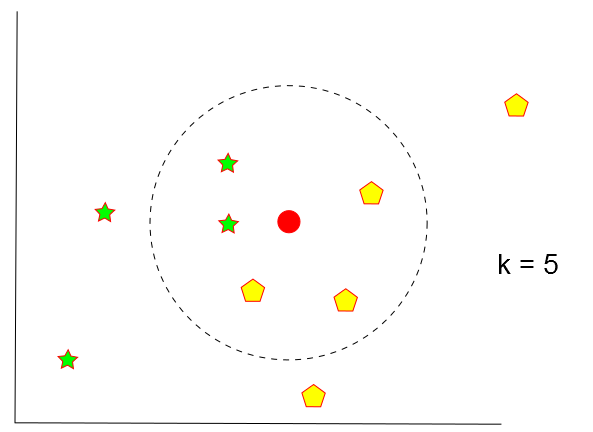
\includegraphics[keepaspectratio=true, scale=0.3]{neigh_small}
	\end{center}
	\item Odległo"sć od sąsiada okre"sla się na podstawie odpowiedniej metryki.
\end{itemize}
\end{frame}
\note{Czerwony punkt symbolizuje nowy obiekt \\
Etykiety wektorów ze zbioru uczącego to pięciokąt i gwiazdka \\
Dla $k = 5$ sąsiedztwo składa się z  2 gwiazdek i 3 pięciokątów. Stąd wniosek, że etykietą nowego obiektu będzie pięciokąt. \\
Sąsiedztwo okre"sla się przy pomocy odpowiedniej metryki. W tym przypadku jest to dystans euklidesowy.}

\begin{frame}{Różne rozmiary sąsiedztw}
\begin{center}
	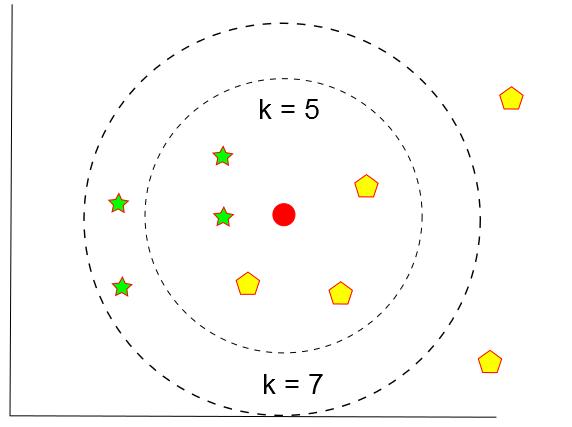
\includegraphics[keepaspectratio=true, scale=0.55]{neigh_k_small}
\end{center}
\end{frame}

\note{Rysunek ilustruje wpływ rozmiaru sąsiedztwa na klasyfikację. \\
Dla $k = 7$ w sąsiedztwie czerwonego punktu znajdują się dodatkowo 2 gwiazdki. \\
Powoduje to, że nowy obiekt otrzyma inną etykietę niż dla $k = 5$.}





